\chapter*{Appendix B}
\addcontentsline{toc}{chapter}{Appendix B}
\label{appB}
An examples of a triangulated surfaces containing ADE singularities.

The surface containing $A_{2+-}$ singularity given by the equation $xz+y^2(x+y+z)=0$
is displayed in the Figure \ref{img:88} at the bottom.

The surface containing $A_{2--}$ singularity given by the equation \newline
$x^2+y^2+z^3+3.2(x^3-3xy^2)=0$
is displayed in the Figure \ref{img:88} at the top.

\begin{figure}[h!]
    \centerline{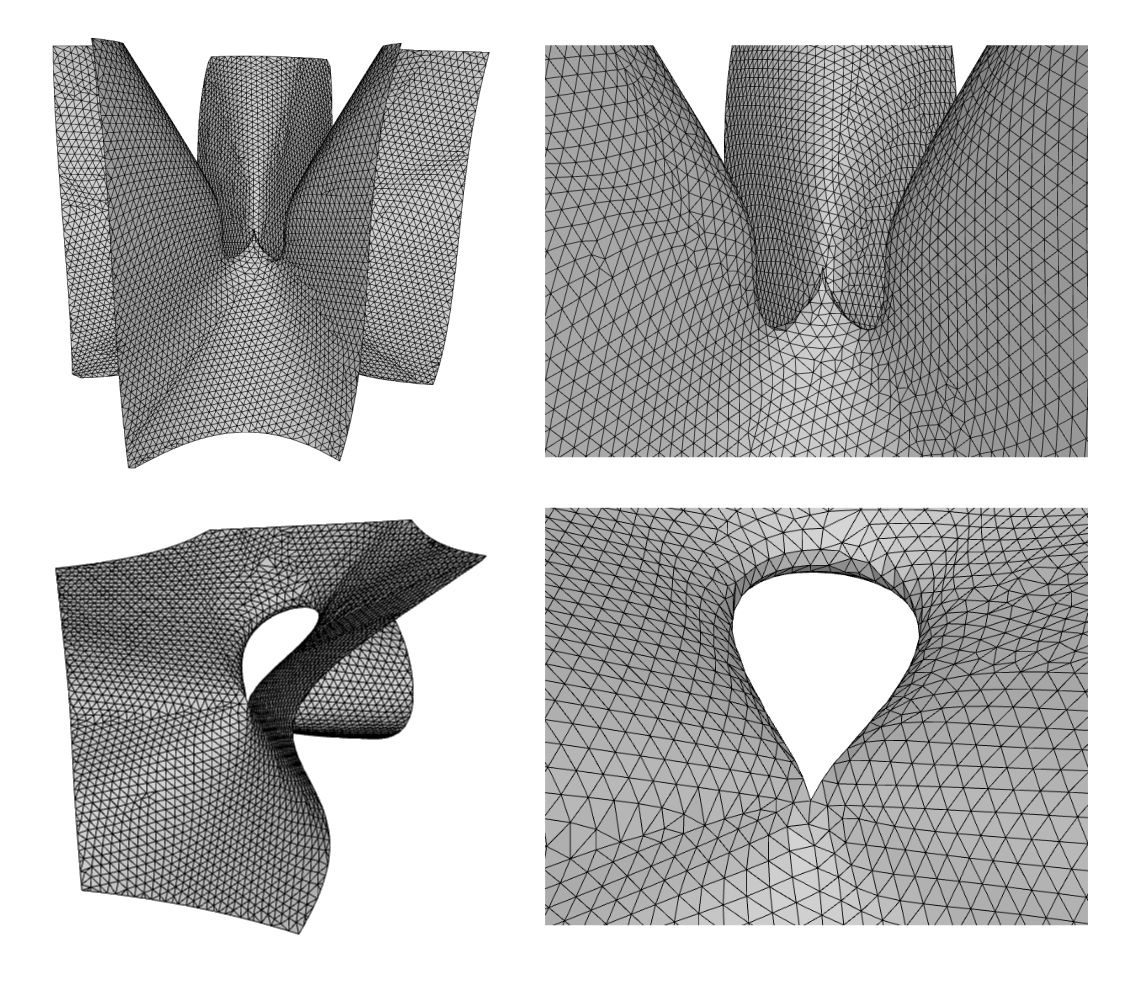
\includegraphics[scale=0.5]{images/img88}}
    \caption[Triangulated surfaces containing ADE singularities]
    {Triangulated surfaces containing ADE singularities.}
    %id obrazku, pomocou ktoreho sa budeme na obrazok odvolavat
    \label{img:88}
\end{figure}

\clearpage
